\documentclass[11pt,largemargins]{homework}

\newcommand{\hwname}{Dwijen Chawra}
\newcommand{\hwemail}{dchawra}
\newcommand{\hwtype}{Homework}
\newcommand{\hwnum}{1}
\newcommand{\hwclass}{CS 251}
\newcommand{\hwlecture}{}
\newcommand{\hwsection}{}

\makeatletter
\renewcommand*\env@matrix[1][\arraystretch]{%
  \edef\arraystretch{#1}%
  \hskip -\arraycolsep
  \let\@ifnextchar\new@ifnextchar
  \array{*\c@MaxMatrixCols c}}
\makeatother

\begin{document}
\maketitle

% Question 1
\newpage
\question
Resources used: None

Collaborators: None

We need to prove that $log(n!) = \Theta(nlog(n))$

This can be done by showing that the upper bound and lower bound are both \(\Theta(nlog(n))\)

We can refactor the original expression to look like so:

$log(n!) = \Theta(log(n^n))$

because 

\begin{align*}
  log(n!) &= log(n(n - 1)(n - 2)...(1)) \\
  &= log(n) + log(n - 1) + log(n - 2) + ... + log(1) \\
\end{align*}

We can see that the above expression is the same as the summation of log(n) from 1 to n.

Similarly, 

% Question 2
\newpage
\question
Resources used: None

Collaborators: None

a)

Base case: $F_13 = 233$, $F_14 = 377$

Inductive hypothesis: For all $n \geq 13$, $F_n \geq 2^{0.6n}$ and $F_{n - 1} \geq 2^{0.6(n - 1)}$

Inductive step:

\begin{align*}
  F_{n + 1} &= 2^{0.6(n + 1)} \\
  F_n + F_{n - 1} \geq F_{n + 1} \\
  \intertext{We can infer that the minimum value of FN and F n-1 is greater than or equal to the value of F n+1.} \\
  2^{0.6n} + 2^{0.6(n - 1)} &\geq 2^{0.6(n + 1)} \\
  2^{0.6} + 1 &\geq 2^{0.6 \cdot 2} \\
  2.52... &\geq 2.3... \\
\end{align*}

We have proven the hypothesis with strong induction.
\vspace{5mm}
\hrule
\vspace{5mm}

b)

Base case: $F_0 = 0$, $F_1 = 1$

Inductive hypothesis: For all $n \geq 0$, $F_n \leq 2^{0.7n}$ and $F_{n - 1} \leq 2^{0.7(n - 1)}$

Inductive step:

\begin{align*}
  F_{n + 1} &= 2^{0.7(n + 1)} \\
  F_n + F_{n - 1} \leq F_{n + 1} \\
  \intertext{We can infer that the maximum value of FN and F n-1 is less than or equal to the value of F n+1.} \\
  2^{0.7n} + 2^{0.7(n - 1)} &\leq 2^{0.7(n + 1)} \\
  2^{0.7} + 1 &\leq 2^{0.7 \cdot 2} \\
  2.62... &\leq 2.63... \\
\end{align*}


We have proven the hypothesis with strong induction.

% Question 3
\newpage
\question
Resources used: None

Collaborators: None

Base Case: 2, $T(2) = 2log_2(2) = 2$

Inductive hypothesis: For all $k > 0$, $T(n) = nlog(n)$ if $n = 2^k$

Inductive step:

\begin{align*}
  T(2^{k+1}) &= 2T(2^{k+1}/2) + 2^{k+1} \\
  &= 2T(2^{k+1}/2^1) + 2^{k+1} \\
  &= 2T(2^k) + 2^{k+1} \\
  \text {Replace $T(2^k)$ with $2^klog(2^k)$} \\
  &= 2(2^klog(2^k)) + 2^{k+1} \\
  &= 2^{k+1}log(2^k) + 2^{k+1} \\
  &= 2^{k+1}(log(2^k) + 1) \\
  &= 2^{k+1}log(2^{k+1}) \\
\end{align*}

We have proven the hypothesis with induction.



% Question 4
\newpage
\question
Resources used: None ---- Collaborators: None

\begin{alphaparts}
  \questionpart

  21 compares, 21 swaps.

  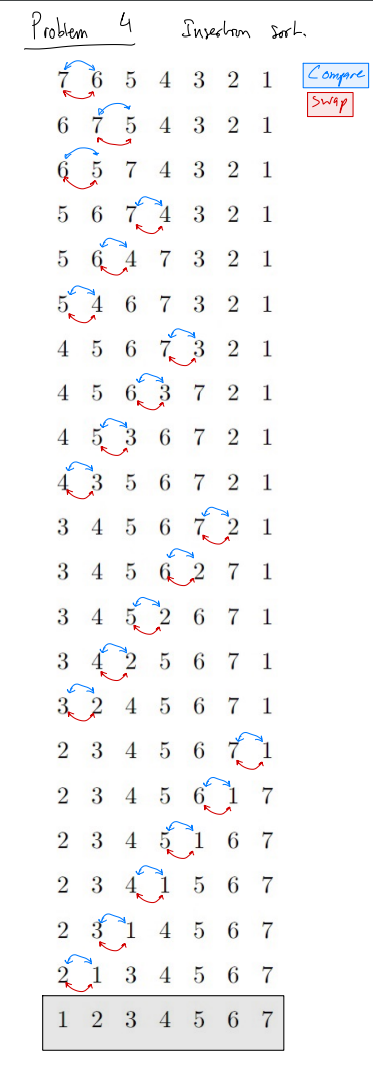
\includegraphics[width=0.4\textwidth]{hw1drawings/4a.png}

  \newpage
  \questionpart
  The number of swaps and compars for Insertion sort on an array [n, n - 1, ..., 2, 1] would be as follows:

  For first element, its compared to the previous, which results in 1 compare and one swap. The next one is
  compared to the previous two, which results in 2 compares and 2 swaps. This can be written with a summation.

  \begin{align*}
    \sum_{i = 1}^{n - 1} i &= \frac{n(n - 1)}{2} \\
    &= \frac{n^2 - n}{2} \\
    &= \frac{n^2}{2} - \frac{n}{2}
  \end{align*}

  For swaps it is the exact same thing, since every compare results in a swap.
  
  \newpage
  \questionpart
  21 compares, 3 swaps.

  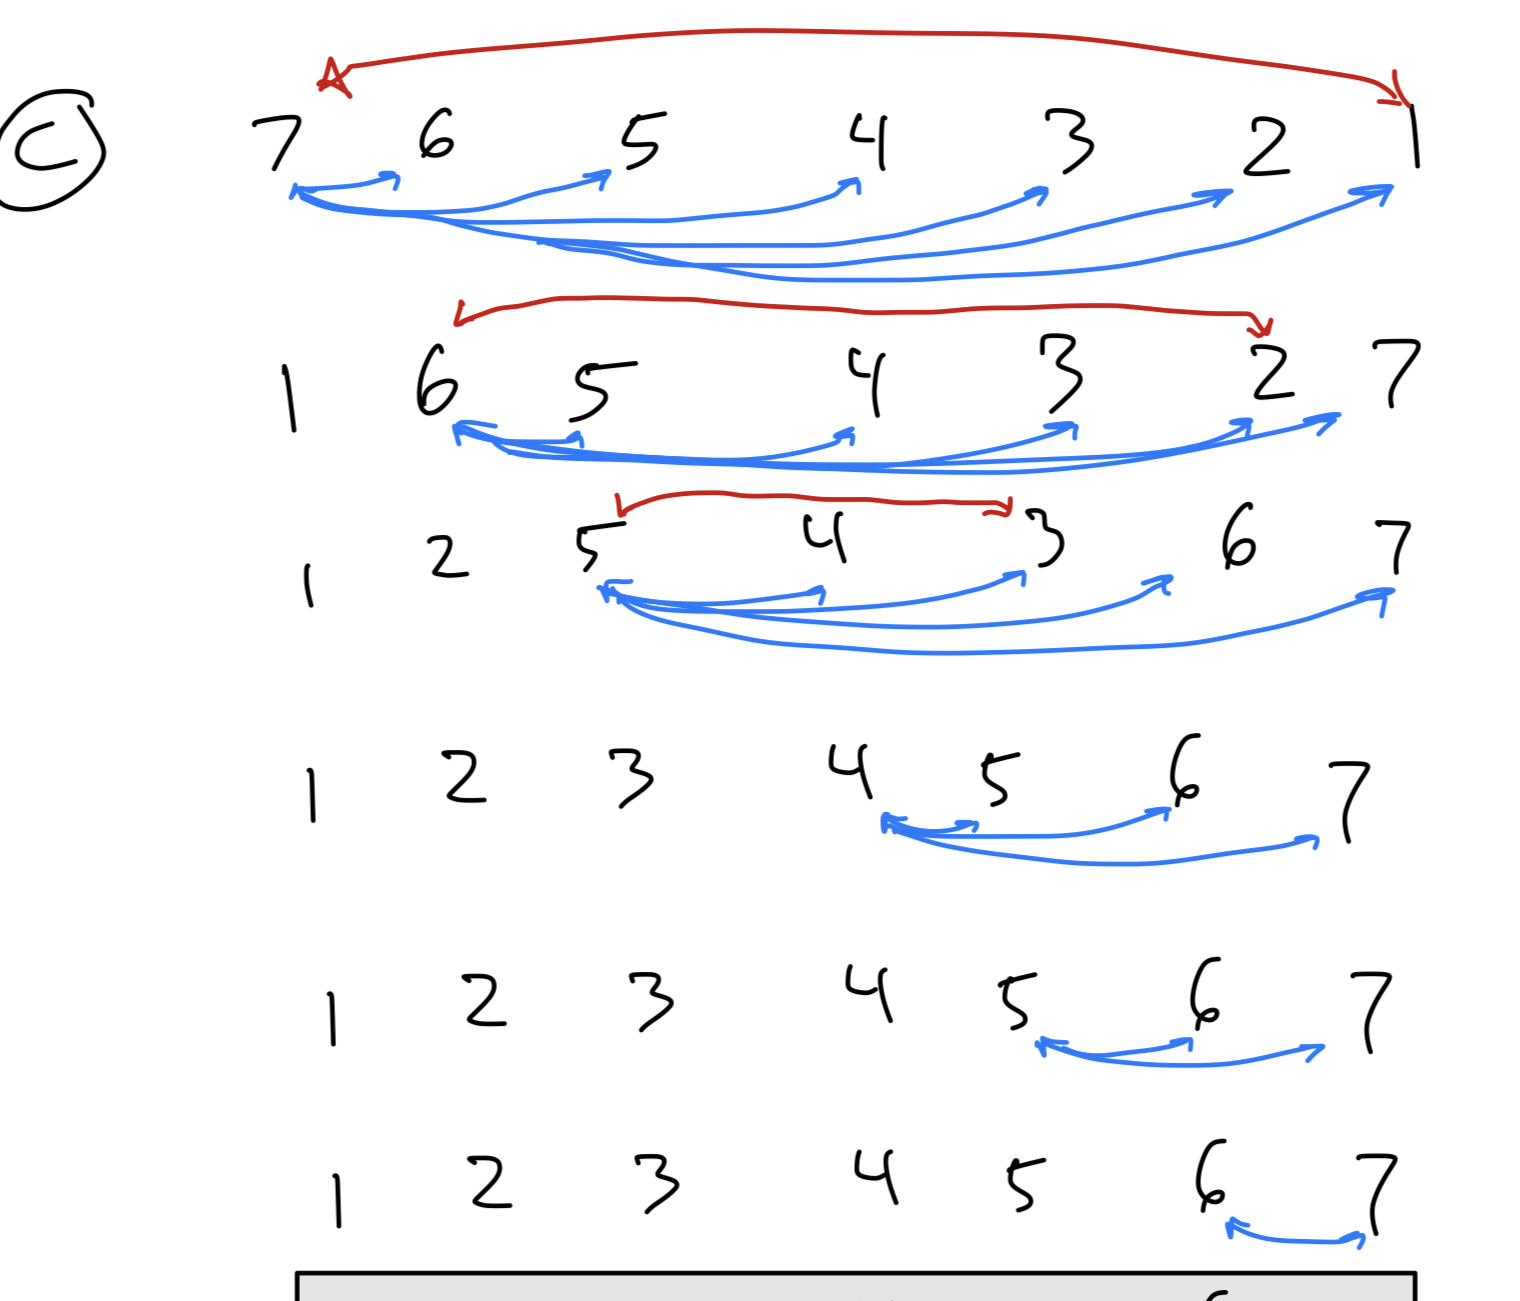
\includegraphics[width=0.4\textwidth]{hw1drawings/4c1.png}

  \newpage
  \questionpart
  Selection sort on an array [n, n - 1, ..., 2, 1] would have compares and swaps like this:

  First run: Compares all elements from n to 1 to find the smallest one - n compares.
  Swaps the smallest element with the first element - 1 swap.

  Second run - n - 1 compares, 1 swap.

  The summation for compares:

  \begin{align*}
    \sum_{i = 1}^{n - 1} i &= \frac{n(n - 1)}{2} \\
    &= \frac{n^2 - n}{2} \\
    &= \frac{n^2}{2} - \frac{n}{2}
  \end{align*}

  The summation for swaps is just n, because every run only has one swap, the smallest element to it's correct position.

  \newpage
  \questionpart
  49 compares, 33 swaps

  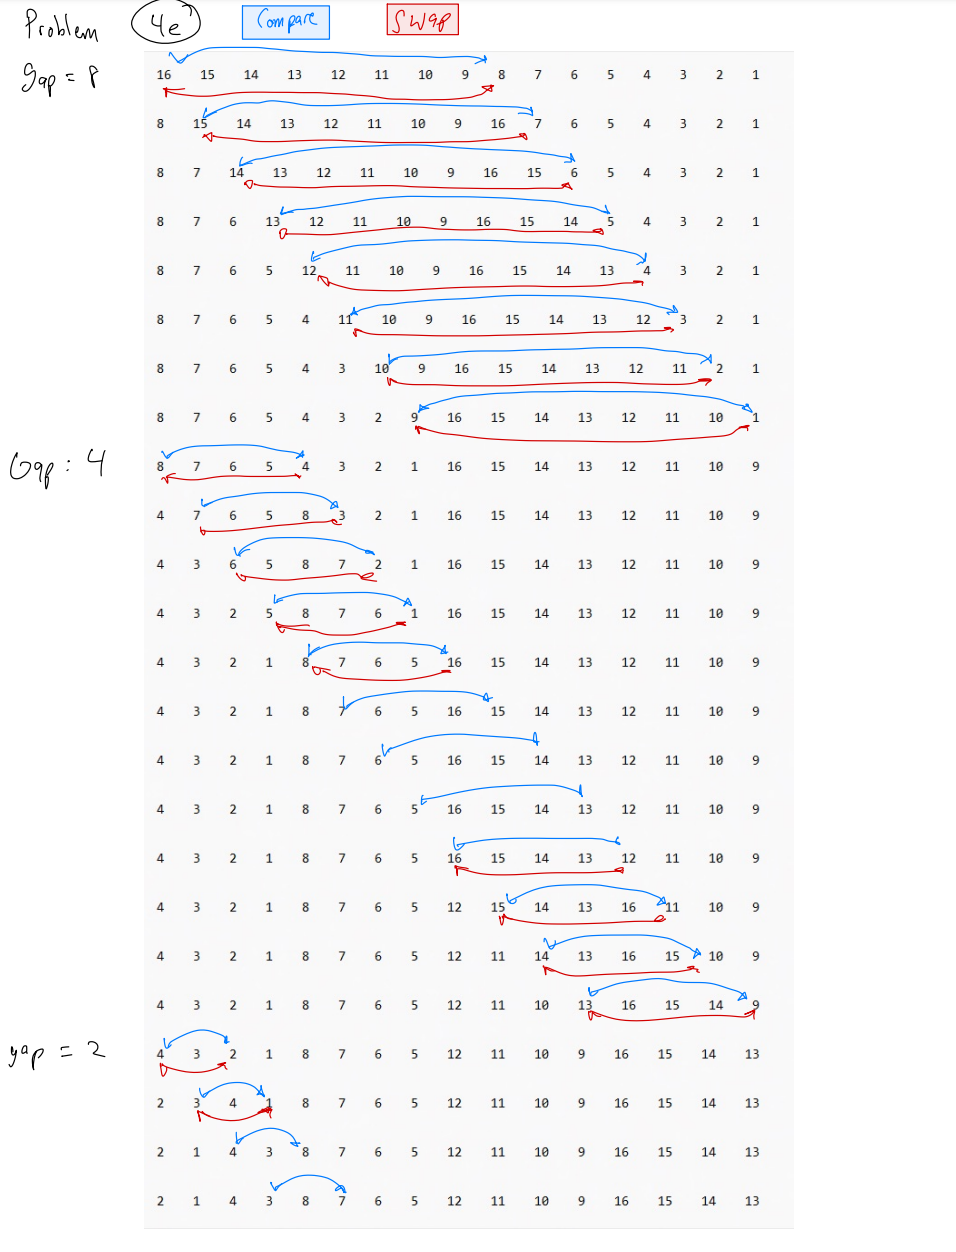
\includegraphics[width=1\textwidth]{hw1drawings/4e1.png}
  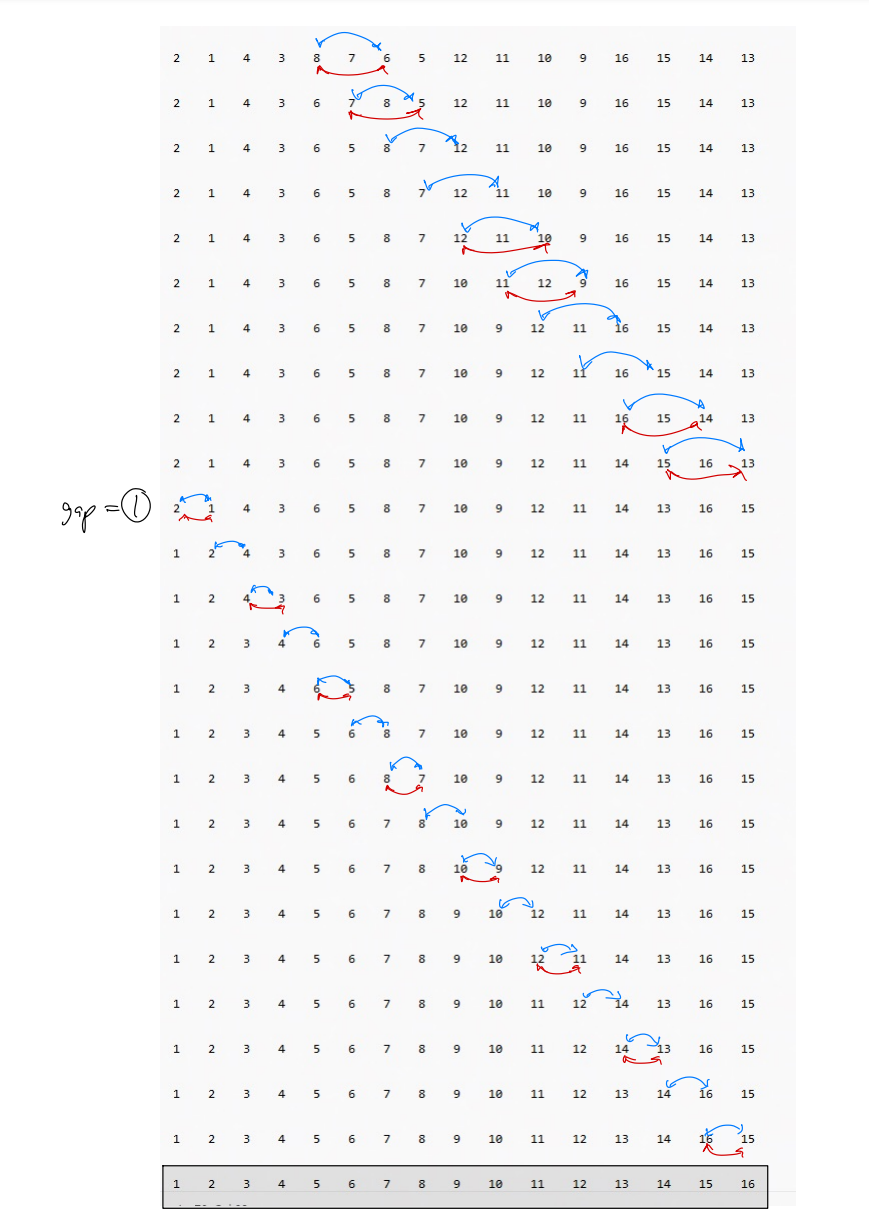
\includegraphics[width=1\textwidth]{hw1drawings/4e2.png}

  \newpage
  \questionpart

  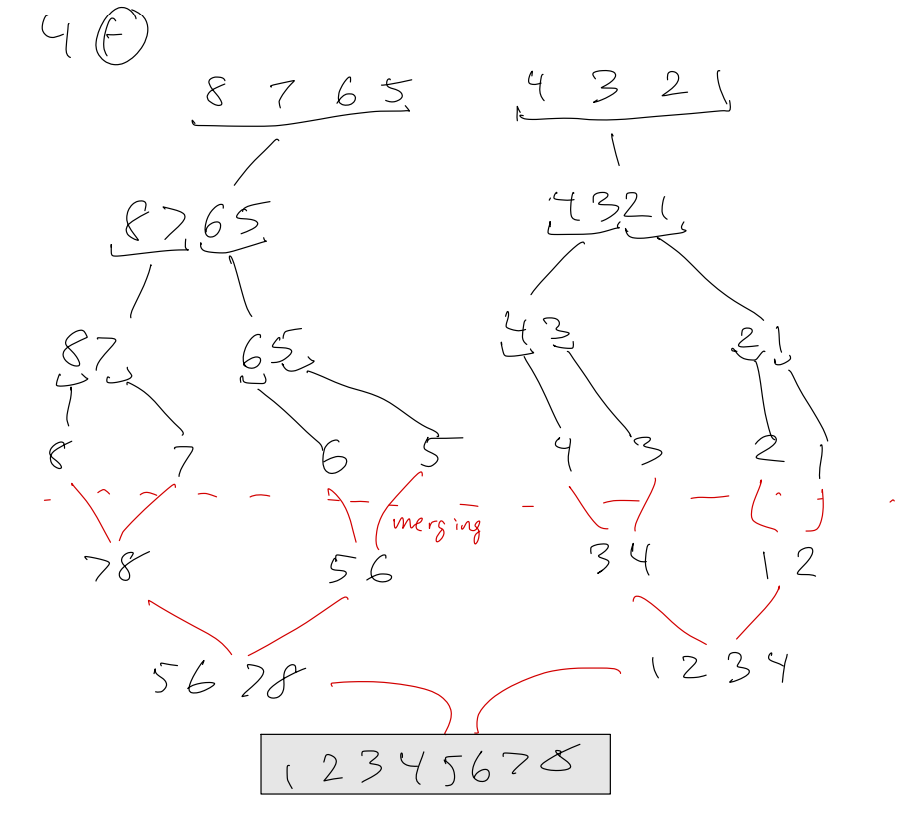
\includegraphics[width=1\textwidth]{hw1drawings/4f.png}


\end{alphaparts}



% Question 5
\newpage
\question
Resources used: None

Collaborators: None

\begin{alphaparts}
  \questionpart

  Inversion pairs:

  (0, 4), (1, 4), (2, 3), (2, 4), (3, 4) - 5 pairs

  \questionpart

  A reversed array has the most inversions. It has n(n - 1)/2 inversions.

  \questionpart

  As inversion count increases, the runtime for insertion sort increases, Insertuion sort is based on swapping a previous 
  larger item with a smaller item that is after. The more inversions, the more swaps.

  \questionpart
  Runtime analysis: It is the exact same as mergesort, because the only overhead that we are adding is memory related. The

  Using the hint in the bottom of the question, I used the algorithm written in the slides and modified it for this purpose.

  \begin{alltt}
algorithm MergeSort(A, l, r)
  inversions = 0                      // this is the inversion counter 
                                      // that will be incremented.
  if (l < r)
    m = (l + r) / 2
    inversions += MergeSort(A, l, m)
    inversions += MergeSort(A, m + 1, r)
    inversions += merge(A, l, m, r)
  end if

  return A, inversions
end algorithm


algorithm merge(A, l, m, r)
  n1 = m – l + 1
  n2 = r – m
  
  inv = 0 // counter for inversions
  
  let L be an array of size n1 + 1
  let R be an array of size n2 + 1

    for (i = 0 to n1 – 1)
      L[i] = A[l + i]
    end for

    for (j = 0 to n2 - 1)
      R[j] = A[m + j + 1]
    end for

    L[n1] = \(\infty\), R[n2] = \(\infty\)
    i = 0, j = 0

    for (k = l to r - 1)
      if (L[i] <= R[j])
        A[k] = L[i]
        i = i + 1
      else                  // this is the inversion
        A[k] = R[j]         // case, when right > left
        j = j + 1
        inv += 1
      end if
    end for

  return A, inv
end algorithm
\end{alltt}

\end{alphaparts}


\end{document}
